\documentclass[a4paper, parskip=half]{scrartcl}
%\usepackage{libertine}
\usepackage[english]{babel}
\usepackage[utf8]{inputenc}
\usepackage[T1]{fontenc}
\usepackage{amsmath}
\usepackage{tikz}
\usepackage{amsthm}
\usepackage{amssymb}
\usepackage{xfrac}
\usepackage[hidelinks]{hyperref}
\usepackage[super]{nth}
\usetikzlibrary{matrix,calc,3d}
\usetikzlibrary{arrows}
\usetikzlibrary{positioning}
\usepackage{float}

\usepackage{csquotes} 
\usepackage[backend=bibtex8,style=numeric]{biblatex} 
\addbibresource{thesis.bib}

\title{Proton Dynamics in Cavities}
\author{Dominik Wille}

\newcommand{\person}[1]{%
	\textsc{#1}%
}

\newcommand{\effect}[1]{%
	\textbf{#1}%
}

\newcommand{\myImage}[2]{
	\begin{figure}[H]
	\centering
	\includegraphics[width = 0.9\textwidth]{img/#1}
	\caption{#2}
	\label{pic:#1}
	\end{figure}
}

\newcommand{\diff}{\mathop{}\!\mathrm{d}}

\newcommand{\myFigRef}[1]{\textit{\hyperref[#1]{Figure \ref*{#1}}}}

\newcommand{\myEqRef}[1]{\textit{\hyperref[eq:#1]{Equation \ref*{eq:#1}}}}

\newcommand{\myEqLabel}[1]{\label{eq:#1}}

\newcommand{\myEqAnnex}[1]{\;\;\;\ast \myEqLabel{#1}}

\newcommand{\myCite}[1]{\footnote{\cite{#1} \citeauthor{#1} \citetitle{#1} \citeyear{#1}}}

\begin{document}
\maketitle

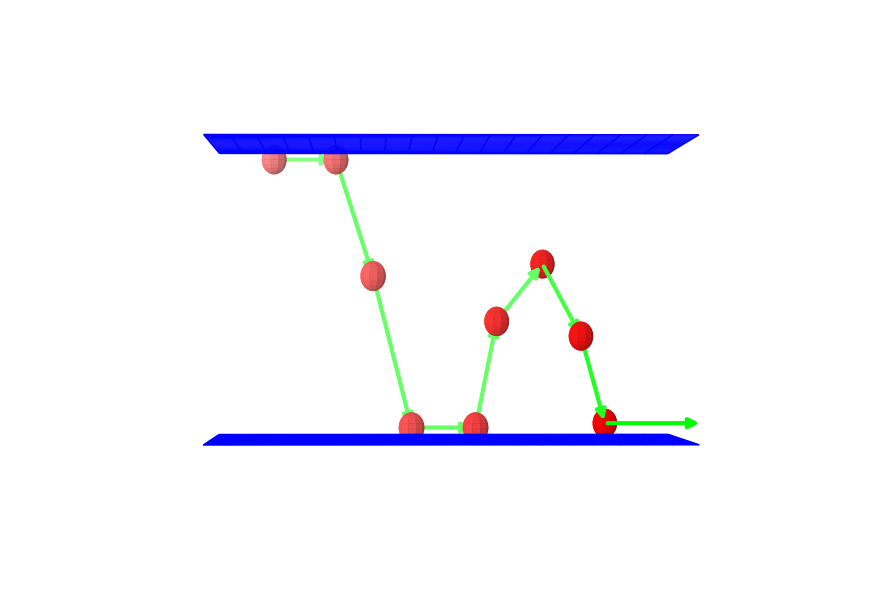
\includegraphics[width=\textwidth]{img/title}

\vfill

\enlargethispage{2cm}
  \parbox[t]{0.45\textwidth}{%
   Freie-Universität-Berlin\\
   Department of Physics\\
   AG Netz
  }
  \parbox[t]{0.55\textwidth}{\raggedleft%
    \nth{1} reviewer: Prof. Dr. Roland R. Netz
  }

\thispagestyle{empty}
\newpage
\tableofcontents
\thispagestyle{empty}
\newpage
% \setcounter{page}{1}

\section{Introduction}
Proton- or generally ion dynamics in fluids directly imply fluctuations in the potential and conductivity of surrounded nano--scaled structures. The major processes which influence these measurable properties and which are considered here are \effect{absorption} and \effect{desorption} processes. The amount of mobile ions which are contained in the fluid are proportional to the fluids conductivity. An experimental way to detect this conductivity is by measuring the ionic current. And since ions carry charges, absorption of ions causes changes of the potential.

Since such fluctuations, could bring hints to extract physical, chemical or even geometrical information concerning the system, they are part of current investigations. Just now some of these fluctuations are the topic of current research\myCite{pinknoise}. 

In this document the motion of one particle is considered as a brownian motion. Even though ions and especially protons are not necessarily smaller than the fluid molecules which is the reason why the diffusion constant does not fulfill \person{Einsteins} formula\myCite{brownian}, the general assumption that the motion is caused by random strokes is fulfilled for smaller particles as well. In this document a \effect{Langevin-Simulation} of a particle is used to determine correlations of the absorption--desorption processes, which can be indirectly measured as conductivity and potential.

The simulations are based on previous analytic calculations by \person{Roland Netz} which obtain these correlation functions for infinite cylindrical and planar geometries\myCite{netzpaper}. To determine the correctness of the \effect{Langevin-Simulation} it is tested for these limiting cases as well as simple simulations for a free particle. Moreover the most important processes which take effect in the correlation functions and methods to describe and implement these in the simulation are briefly summarized and explained.

The title image shows one visualized particle on a random walk between two plates in 2-d for different times. The time increases from left to right. 

\newpage
\section{Analytic calculations}
The analytic calculations are mostly inherited from \cite{netzpaper} and \cite{netzpaper2}. To understand the used properties in the simulation later on, the key principles should be explained briefly.

Considered should be $N$ charges carriers such as ions or protons. For every particle $i\in\left\lbrace 1,2,...,N \right\rbrace$ the binary function $n_j^i(t)$ should stand for the absorption state of the particle on the surface $j$. $n_A^i(t) = 1$ if the particle is absorbed on Plate $A$ and $n_A^i(t) = 0$ if it is not.

Of course the number of particles absorbed on plate $A$ is given by:

\begin{align}
N_A(t) = \sum_{i=1}^N n_A^i(t)
\end{align}

Since experimental investigation measure fluctuations in the potential of nano--structures, especially the auto--correlation function of $N_A(t)$, is of essential importance.

\begin{align}
\langle N_A(0) N_A(t)\rangle &= \sum_{i,j = 1}^N \langle n_A^i(0) n_A^j(t)\rangle\\
&= \sum_{i \neq j}^N \langle n_A^i(0) n_A^j(t)\rangle + \sum_{i =1}^N \langle n_A^i(0) n_A^j(t)\rangle
\end{align}
The particles are usually uncorrelated among each other 
\begin{align}
\langle n_A^i(0) n_A^j(t)\rangle = \langle n_A(0) \rangle\langle n_A(t) \rangle
\end{align}
so let the expectation value of the absorption state for an single particle be:
\begin{align}
\langle n_A^i(t) \rangle &= \langle n_A^i(0) \rangle = p_A \\
\Rightarrow \langle N_A(0) N_A(t)\rangle &= N(N-1)p_a^2 + N\langle n_A(0) n_A(t)\rangle
\end{align}
The only non--trivial quantity to calculate can be defined via the singe--ion correlation function $C_{AA}(t)$ which is the probability that a particle is absorbed at time $t$ given it is absorbed at time $t=0$.
\begin{align}
C_{AA}(t) &= \langle n_A(0) n_A(t) \rangle / \langle n_A(0) \rangle \\
\Rightarrow \langle N_A(0) N_A(t)\rangle &= N^2p_a^2 + Np_AC_{AA}(t) - Np_a^2
\end{align}

\subsection{Constructing the single--ion correlation function}
\subsubsection{One surface}
For a single surface $A$, one particle that is absorbed at time $t=0$ can basically keep absorbed until time $t$ or desorb $n$--times before it is absorbed again, if it should be absorbed at time $t$. 
\begin{figure}[H]
\centering
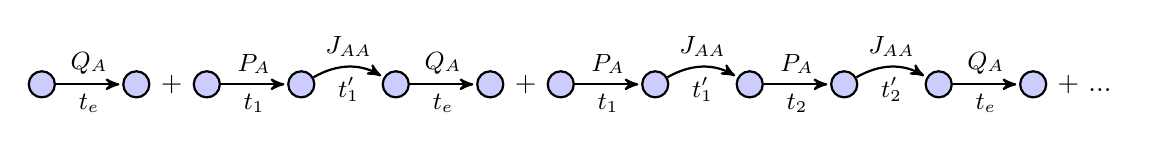
\begin{tikzpicture}[->,>=stealth',shorten >=1pt,auto,node distance=1.2cm,
  thick,main node/.style={circle,fill=blue!20,draw,font=\sffamily\bfseries}]

  \node[main node] (5) {};
  \node[main node] (6) [right of=5] {};
  \node (7) [right=0.0cm of 6] {$+$};

  \path[every node/.style={font=\sffamily\small}]
    (5) edge node [above] {$Q_A$} node [below] {$t_e$} (6);


  \node[main node] (1) [right=0.0cm of 7] {};
  \node[main node] (2) [right of=1] {};
  \node[main node] (3) [right of=2] {};
  \node[main node] (4) [right of=3] {};

  \path[every node/.style={font=\sffamily\small}]
    (1) edge node [above] {$P_A$} node [below] {$t_1$} (2)
    (2) edge[bend left] node[above] {$J_{AA}$} node [below] {$t_1'$} (3)
    (3) edge node [above] {$Q_A$} node [below] {$t_e$} (4);
    
  \node (8) [right=0.0cm of 4] {$+$};
  \node[main node] (9) [right=0.0cm of 8] {};
  \node[main node] (10) [right of=9] {};
  \node[main node] (11) [right of=10] {};
  \node[main node] (12) [right of=11] {};
  \node[main node] (13) [right of=12] {};
  \node[main node] (14) [right of=13] {};
  
  \path[every node/.style={font=\sffamily\small}]
    (9) edge node [above] {$P_A$} node [below] {$t_1$} (10)
    (10) edge[bend left] node[above] {$J_{AA}$} node [below] {$t_1'$} (11)
    (11) edge node [above] {$P_A$} node [below] {$t_2$} (12)
    (12) edge[bend left] node[above] {$J_{AA}$} node [below] {$t_2'$} (13)
    (13) edge node [above] {$Q_A$} node [below] {$t_e$} (14);
    
  \node (15) [right=0.0cm of 14] {$+$ ...};

\end{tikzpicture}
\caption{Illustrated construction of $C_{AA}(t)$}
\label{fig:ways}
\end{figure}
As illustrated in the figure above $C_{AA}(t)$ as the sum of different paths. The distribution $P(t)$ is the Probability for an absorbed ion to desorb at time $t$ for the first time. $Q_A(t)$ is the survival distribution for an ion to be absorbed on the surface $A$ over the time span $t=0$ to $t$. Note that this equals the probability that ion desorbes at some time $> t$.It is given by:
\begin{align}
Q_A(t) = \int_t^\infty P(t') \diff t'
\end{align}
$J_{AA}(t)$ is the probability for an ion to desorb at time $t=0$ and to return to the surface $A$ at time $t$.

The probability that a particle is absorbed at time $t$ given it is absorbed at time $t=0$ is the sum over the probabilities of all ways on which a particle is absorbed at time $t=0$ and on time $t$. The probability of one way on the other hand is the product of the probabilities of its parts $Q_A$, $P_A$, and $J_{AA}$.

Generally all that stages in $C_{AA}(t)$ of particles could have every time $<t$. Therefore it is necessary to vary all these times. 

The construct of $C_{AA}$ below sums up all variations illustrated in \myFigRef{fig:ways} with general times $t_e$ for $Q(t)$, $t_j$ for $P_A(t)$ and $t_j'$ for $J_{AA}(t)$. In order to obtain the probability at time $t$ the \effect{Dirac-Delta-Function} pics out variants with $\sum_{j} (t_j+t_j') + t_e = t$.

\begin{align}
C_{AA}(t) = &\sum_{i=0}^\infty \Bigg\lbrace \int_0^\infty \diff t_e\, Q_A(t_e) \prod_{j=1}^i \left[ \int_0^\infty \diff t_j\, P_A(t_j) \int_0^\infty \diff t_j'\, J_{AA}(t_j')\right]\notag\\ 
&\delta \left(\sum_{k=1}^i(t_k+t_k') + t_e - t \right) \Bigg\rbrace \myEqLabel{def_Caa}
\end{align}

This construct itself is very though to analyze. But there is common trick to derive the \effect{Laplace-transform} $\widetilde{C}_{AA}(\omega)$ of $C_{AA}(t)$.

\begin{align}
\widetilde{C}_{AA}(\omega) &= \int_0^\infty e^{-\omega t'} \cdot C_{AA}(t') \diff t'
\end{align}

Remember that the integrand in \myEqRef{def_Caa} has only non--zero values for $\sum_{j} (t_j+t_j') + t_e = t$. Therefore it is possible to split the $e^{-\omega t'}$--term.

\begin{align}
e^{-\omega t'} &= e^{-\omega t_e} \cdot \prod_{j=1}^i e^{-\omega t_j} \cdot e^{-\omega t_j'}\\
\Rightarrow  \widetilde{C}_{AA}(\omega) &= \sum_{i=0}^\infty \Bigg\lbrace \int_0^\infty \diff t_e\, e^{-\omega t_e} Q_A(t_e) \prod_{j=1}^i \left[ \int_0^\infty \diff t_j\, e^{-\omega t_j} P_A(t_j) \int_0^\infty \diff t_j'\, e^{-\omega t_j'} J_{AA}(t_j')\right]\notag\\ 
&\delta \left(\sum_{k=1}^i(t_k+t_k') + t_e - t \right) \Bigg\rbrace\\
&= \sum_{i=0}^\infty \Bigg\lbrace \widetilde{Q}_A(\omega) \prod_{j=1}^i \left[\widetilde{P}_A(\omega) \cdot \widetilde{J}_{AA}(\omega) \right]  \Bigg\rbrace \\
&= \sum_{i=0}^\infty \widetilde{Q}_A(\omega) \left[\widetilde{P}_A(\omega) \cdot \widetilde{J}_{AA}(\omega) \right]^i
\end{align}
With the formula for geometric series 
\begin{align}
\sum_{i=0}^{n-1}q^i = \frac{1-q^n}{1-q} 
\end{align}
this becomes the following expression:
\begin{align}
\widetilde{C}_{AA}(\omega) &= \frac{\widetilde{Q}_A(\omega)}{1-\widetilde{P}_A(\omega) \cdot \widetilde{J}_{AA}(\omega)}
\end{align}
\subsubsection{Two surfaces}
The calculation of $\widetilde{C}_{AA}(\omega)$ for one surface should give a general idea how the laplace-transform of The correlation functions look like.

For instance $\overline{C}_{AA}(\omega)$, $\overline{C}_{BB}(\omega)$ which omit the $\widetilde{Q}_{A/B}(\omega)$ terms, represent ways where the particle is absorbed at time $t=0$ and exactly absorbs at time $t$. 
\begin{align}
\overline{C}_{AA}(\omega) &= \frac{1}{1-\widetilde{P}_A(\omega) \cdot \widetilde{J}_{AA}(\omega)} \\
\overline{C}_{BB}(\omega) &= \frac{1}{1-\widetilde{P}_B(\omega) \cdot \widetilde{J}_{BB}(\omega)} 
\end{align}

Parts which are performed one time are in the nominator, parts which are performed $n$--times are in the denominator. Parts which are performed equal times can be just multiplied in the laplace-transform.

$\widetilde{C}_{AA}(\omega)$ can be constructed as:

\begin{align}
&\widetilde{C}_{AA}(\omega) = \frac{\overline{C}_{AA}(\omega) \, \widetilde{Q}_{A}(\omega)}{1-\overline{C}_{AA}(\omega)\, \widetilde{P}_A(\omega)\, \widetilde{J}_{AB}(\omega)\, \overline{C}_{BB}(\omega)\, \widetilde{P}_B(\omega)\,\widetilde{J}_{BA}(\omega)}\\
&= \frac{\widetilde{Q}_A(\omega)\left(1 - \widetilde{P}_A(\omega)\, \widetilde{J}_{AA}(\omega) \right)}{\left(1 - \widetilde{P}_A(\omega)\, \widetilde{J}_{AA}(\omega) \right)\left(1 - \widetilde{P}_B(\omega)\, \widetilde{J}_{BB}(\omega) \right) - \widetilde{P}_A(\omega)\, \widetilde{J}_{AB}(\omega)\, \widetilde{P}_B(\omega)\, \widetilde{J}_{BA}(\omega)}
\end{align}
\subsection{Limiting case}

\newpage
\section{Brownian Dynamics}
The motion of a particle such as a proton in a fluid is primarily  caused by collisions with other particles. This motion firstly was described by \person{Robert Brown} who observed the motion of minute particles of pollen in water and is widely known as \effect{brownian motion}.
\subsection{Langevin Symulation}
\subsubsection{Priciple}
The principle of a Langevin simulation generally is to consider collisions with other particles as a random force. And propergate the position of a particle over small time steps $\delta t$.
\subsubsection{Physical background}
An approach to describe situations with brownian motion was suggested by \person{Paul Langevin} who added the random force $\mathbf{Z}(t)$ in newtons equation of motion. This stochastic term represents the collision driven force. His equation, the Langevin equation reads:

\begin{align}
m \ddot{\mathbf{r}} = -\lambda\dot{\mathbf{r}} + \mathbf{Z}(t)
\end{align}

where $m$ is the mass of the particle, $\mathbf{r}$ the position of the particle and $\lambda$ The friction constant.

Brownian dynamics can be represented with the so called \effect{overdamped langevin equation} where the $m \ddot{\mathbf{r}}$ term is neglected. The equation for the prevailing situation therefore is:

\begin{align}
\lambda\dot{\mathbf{r}} = \mathbf{Z}(t)
\end{align}

In order to get an iterable expression this expression is discretesated in time intervals $\Delta t$:

\begin{align}
\int_t^{t+ \delta t} \dot{\mathbf{r}}(t')\, dt' &= \int_t^{t+ \Delta t} \frac{\mathbf{Z}(t')}{\lambda}\, dt' \\
\mathbf{r}(t + \delta t) - \mathbf{r}(t) &= \frac{1}{\lambda} \int_t^{t+ \Delta t} \mathbf{Z}(t)\, dt'\\
\mathbf{r}(t + \delta t) - \mathbf{r}(t) &\cong \boldsymbol{\zeta}(t, \varepsilon)
\end{align}

In the discussed 1--dimensional case $\varepsilon$ is the mean step size and $\boldsymbol{\zeta}(t, \varepsilon)$ is one random vector. For a simple random walk with unique step size this will be $\varepsilon$ or $-\varepsilon$ with a chance of $50\%$ each. For a gaussian random walk this will be some value $s$ with a probability:

\begin{align}
P(s) = \frac{1}{\varepsilon \sqrt{2\pi}} e^{-\sfrac{s^2}{2\varepsilon^2}}
\end{align} 

The position of a particle at time $t + \Delta t$ can easily derived from its position at time $t$.

\begin{align}
\mathbf{r}(t + \delta t) = \mathbf{r}(t) + \boldsymbol{\zeta}(t, \varepsilon)
\end{align}

\subsection{Connection to diffusion}
The probability density function for both mentioned types of \effect{random walks} fulfill the diffusion equation (\textit{Note: }$n = \sfrac{t}{\delta t}$):
\begin{align}
\frac{\partial}{\partial t} \rho(x,t) &= D \frac{\partial^2}{\partial x^2 } \rho(x,t) \myEqAnnex{diffusion_PDE} \\
\mathrm{with} \, \, \,\, D &= \frac{\varepsilon^2}{2 \delta t} \myEqLabel{def:D}
\end{align}
What means that a random walk can also be seen as a diffusion process. The exact form of the probability density functions is discussed below.
\subsubsection{Fixed step size}
The motion which is performed in the langevin simulation is widely known as a \effect{random walk}. The simplest variant is as mentioned before to choose $\varepsilon$ or $-\varepsilon$ with a chance of $50\%$ each. The probability $p(x, n)$ that a random walk with discrete steps of length $\varepsilon$ comes to a position $x$ after $n$ steps. Is given by:

\begin{align}
p(x, n) = \frac{\mathrm{Number\, of\, ways\, to\, position\,} x}{\mathrm{Total\, number\, of\, ways}} = \frac{N_x}{N}
\end{align}

Since there are 2 possible successors for every position the total number of ways  doubles every step.

\begin{align}
N = 2^n
\end{align}

The number of ways to the position $x$ after n steps can be obtained by \effect{Pascal's triangle}.

\begin{figure}[H]
\centering
\begin{tikzpicture}[description/.style={fill=white,inner sep=2pt}]
\matrix (m) [matrix of math nodes, row sep=1.5em,
column sep=0.3em, text height=1.5ex, text depth=0.25ex,
nodes={
        minimum width=1.0cm
    },
]
{%
\mathrm{Step/Position} &-3\varepsilon &-2\varepsilon & -1\varepsilon & 0 & \varepsilon & 2\varepsilon &3\varepsilon \\
0 & & & & 1 & & & \\
1 & & & 1 & & 1 & & \\
2 & & 1 & & 2 & & 1 &\\
3 & 1 & & 3 & & 3 & & 1\\};
\path[-] (m-2-5) edge (m-3-4)
		 (m-2-5) edge (m-3-6)
		 (m-3-4) edge (m-4-5)
		 (m-3-4) edge (m-4-3)
		 (m-3-6) edge (m-4-7)
		 (m-3-6) edge (m-4-5)
		 (m-5-6) edge (m-4-5)
		 (m-5-4) edge (m-4-3)
		 (m-5-8) edge (m-4-7)
		 (m-5-6) edge (m-4-5)
		 (m-5-6) edge (m-4-5)
		 (m-5-2) edge (m-4-3)
		 (m-5-6) edge (m-4-7)
		 (m-5-4) edge (m-4-5);
\end{tikzpicture}
\caption{Number of ways to different distances}
\end{figure}

\begin{align}
N_x &= \binom{n}{k}\\
\mathrm{with} \, \, \,\, k &= \frac{1}{2}\left(\frac{x}{\varepsilon} + n \right)
\end{align}

Therefore $p(x,n)$ follows as:

\begin{align}
p(x,n) = \binom{n}{k} \cdot 2^{-n}
\end{align}
A consequence of the \effect{de Moivre–Laplace theorem} is that for large numbers of steps $(n\rightarrow\infty)$ this expression can be approximated with the following gaussian curve:

\begin{align}
p(x,n) \cong \sqrt{\frac{2}{n \pi}} e^{-\sfrac{x^2}{2\varepsilon^2 n}} \myEqAnnex{moivre_laplace_theorem}
\end{align}

The probability function $p(x,n)$ has valid values only for values 
\begin{align}
x \in \{x\; |\; x = z \cdot 2 \varepsilon + \varepsilon\, (n\,\mathrm{mod}\, 2),\, z \in \mathbb{Z} \wedge |x| \leq n \varepsilon\} 
\end{align}
For other values $x$ the probability is $0$. This means that there is only one value per $2\epsilon$ interval, therefore the probability density function $\rho(x,n)$ is:
\begin{align}
\rho(x,n) = \frac{1}{2\varepsilon}\; p(x,n) = \frac{1}{\varepsilon\sqrt{2\pi n}} e^{-\sfrac{x^2}{2\varepsilon^2 n}}
\end{align}
Which is the normal distribution with $\mu = 0;\;\; \sigma =  \varepsilon\sqrt{n}$.

\subsubsection{Gaussian random walk}
The probability density function for a gaussian random walk with mean step size $\varepsilon$ has exactly the same form as the for fixed step size $\varepsilon$.
\begin{align}
\rho(x,n) = \frac{1}{\varepsilon\sqrt{2\pi n}} e^{-\sfrac{x^2}{2\varepsilon^2 n}} \myEqLabel{rho_gauss}
\end{align}
This can easily be shown with a mathematical induction for $p(x,n)$. Note that because every position is possible the probability 
\begin{align}
p(x,n) = 0 
\end{align}
because that means that the number of possible positions is infinite.

\textbf{Base case} ($n = 1$)\textbf{:}
\begin{align}
\rho(x,1) = \frac{1}{\varepsilon\sqrt{2\pi}} e^{-\sfrac{x^2}{2\varepsilon^2}}
\end{align}
Which is exactly the expression of a gaussian distributed 1--dimensional random vector with $\varepsilon$ variance. $\checkmark$

\textbf{Inductive step} ($n + 1$)\textbf{:}
\begin{align}
\rho(x,n+1) &= \int_{-\infty}^\infty \frac{1}{\varepsilon\sqrt{2n\pi}}\, e^{-\sfrac{x'^2}{2n\varepsilon^2}} \cdot \frac{1}{\varepsilon\sqrt{2\pi}}\, e^{-\sfrac{(x - x')^2}{2\varepsilon^2}} \diff x'\\
&= \frac{1}{\varepsilon\sqrt{2(n+1)\pi}}\, e^{-\sfrac{x^2}{2(n+1)\varepsilon^2}} \myEqAnnex{gauss_random_walk}
\end{align}

and since the calculated $\rho(x,n+1)$ is the same as $\rho(x,n)$ in \myEqRef{rho_gauss} the expression is proofed. $\checkmark$
\subsection{Mean square distance}
Obviously the expectation value for $x$ after $n$ steps $\langle x_n\rangle = 0$. What can be derived from:
\begin{align}
\langle x_n\rangle = \int_{-\infty}^\infty x \cdot \rho(x,t)\diff x = 0
\end{align}
But the \effect{Mean Square Distance} $\langle x_n^2\rangle$ (MSD) fulfills the following expression:
\begin{align}
\langle x_n^2\rangle = \int_{-\infty}^\infty x^2 \cdot \rho(x,t)\diff x = 2 D t \myEqAnnex{MSD}
\end{align}

\newpage
\section{Free particle - MSD}
A very simple test is to check if the simulation of a particle without any barriers has a linear growing MSD in time steps. \myFigRef{pic:mean_square} shows the average squared distance $x_n^2$ for different numbers of runs compared to the analytic expression. The parameters were:
\begin{center}
\begin{tabular}{c|c}
Parameter & Value \\\hline
$D$ & 0.1 \\
$\delta t$ & 20 \\
$x(n=0)$ & 0 \\
$n_{\mathrm{max}}$ & 400
\end{tabular}
\end{center}
Note that $\varepsilon$ is determined by \myEqRef{def:D}.

The expectation is that for large numbers of runs the mean square converges against the following analytic expression derived from \myEqRef{MSD}:
\begin{align}
\langle x_n^2\rangle (t) &= 2 D t \\
\Rightarrow\langle x_n^2\rangle (n) &= 2 D \delta t \cdot n
\end{align}
\myImage{mean_square}{MSD over time for different numbers of runs}

\newpage
\section{Infinite plates}
The system which is simulated consists of two infinite plates A and B with distance $H$. Between the two plates is some fluid which surrounds the simulated ion. The ion absorbs at the surface of the two plates with the probability $p$ and desorbs with an exponential decaying probability $P(t)$ given by:
\begin{align}
P(t) = \frac{1}{\tau}e^{- \sfrac{t}{\tau}} \myEqLabel{absorb_dist}
\end{align}
\begin{figure}[H]
\centering
\begin{tikzpicture}[scale=.8, z={(-.707,-.3)}]
    \draw (6,0,0) -- (0,0,0);
    \draw (6,0,0) -- (6,0,-3);
    \draw (6,3,-3) -- (6,3,0);
    \draw (6,3,0) -- (0,3,0);
    \draw (0,3,-3) -- (6,3,-3);
    \draw (0,0,-3) -- (6,0,-3);
    \draw (0,0,0) -- (0,0,-3); 
    \draw (0,3,0) -- (0,3,-3);
    \draw (3,0,-1.5) node{B};
    \draw (3,3,-1.5) node{A};
    \draw[arrows=<->] (0,0.2,0) -- (0,2.8,0);
    \draw (-0.3,1.5,0) node{$H$};
\end{tikzpicture}
\caption{Schematic structure of the system}
\end{figure}
\subsection{Simple random walk vs. Gaussian random walk}

For all relevant simulations a gaussian random walk was used. Even if the distribution becomes equivalent for large numbers of steps the gauss distribution represents a much more natural motion of the particle. Moreover much smaller step sizes what means more steps in the simulation are necessary to allow small motions of the particle. And since performance of the simulation is not an issue the gaussian random walk is just superior the simple random walk. Below figures show example random walks between two plates at $x = \pm 1$.

\myImage{fixed_pos}{Position of a particle on a simple random walk}

\myImage{gauss_pos}{Position of a particle on a gaussian random walk}

\subsection{Probability density}
The probability density for two infinite plates where the particle can absorb looks for $t\rightarrow \infty$ is shown in the figure below. The plates are again at $x = \pm 1$.
\myImage{probability_density}{Probability density for two plates}
The exception for a reflecting plate would be a constant probability density function. The given probability density function shows some important differences which may due to the implementation of the surface reaction boundary condition. 

It was implemented that the particle absorbs when it crosses one plate with the probability $p$ which was chosen as $0.3$ here. 
If the particle absorbs it keeps absorbed for an exponential distributed time as \myEqRef{absorb_dist}. After the time the particle keeps absorbed the langevin simulation continues from the point on the plate. If the first step goes through the plate again the particle absorbs again in the next step.

This directly implies that there will be significant probability that the particle is at the position of a plate what causes the very high values at $x = \pm 1$. On the other hand the probability that the particle is next to a plate but not absorbed is significant smaller than that it is somewhere else between the plates. This may due to the implementation of the boundary condition as well because all movements that would crosses a plate end up on the position of the plate here. So ways that would include a reflection process at the boundaries drop out for absorbing plates. 


\subsection{Correlation functions}
For a geometry with two plates there is a an analytic expression for the Correlation functions $C_{AA}(t)$ and $C_{AB}(t)$ which represent the probability for an ion to be absorbed at time $t$ on plate $\mathrm{A}/\mathrm{B}$ given that it is absorbed on plate $\mathrm{A}$ at time $t=0$.

These correlation functions can easily be obtained from the langevin simulation by noting if and where the particle is absorbed over the time. 

Afterwards the values of the correlation function $C_{AA}(t)$ can be calculated as the number of time intervals with length $t$ where the ion is absorbed on plate $\mathrm{A}$ at the beginning and at the end over the total number of intervals.

Similarly the values of the correlation function $C_{AB}(t)$ can be calculated as the number of time intervals with length $t$ where the ion is absorbed on plate $\mathrm{A}$ at the beginning and on plate $\mathrm{B}$ at the end over the total number of intervals.

The correlation functions were obtained out of $1$ simulation. For all correlation functions the values of the correlation function $C(t)$ for different times $t$ were calculated as:

\begin{align}
  C_{ij}(t) = \frac{\int_0^{t_{max}-t} S_i(t') \cdot S_j(t' + t) \diff t'}{\int_0^{t_{max}-t} S_i(t') \diff t'}
\end{align}

Where $S_{i/j}(t) = 1$ if the particle has the state of interest at the beginning/end of an interval and $S_{i/j}(t) = 0$ otherwise.

\subsection{Parameters of the simulation}
The run for the comparison was performed with the following parameters:
\begin{center}
\begin{tabular}{c|c}
Parameter & Value \\\hline
$D$ & 0.1 \\
$\delta t$ & 0.1 \\
$\tau$ & 1.0 \\
$p$ & 1.0 \\
$H$ & 1.0
\end{tabular}
\end{center}

where $D$ the diffusion constant, $\delta t$ the step size, $\tau$ the exponential decay constant for the desorption probability, $p$ the probability that a particle at the boundary absorbs and $s$ is the plate distance. The start position for this lagevin--simulation is not relevant for the correlation functions. 

\subsection{Interpretation}

Also the behavior of the correlation functions in \myFigRef{pic:caa_cab} is easily explainable. Obviously $C_{AA}(t)$ starts from $1$ because after its definition it is definitely absorbed at time $t=0$ on Plate $A$. $C_{AB}(t)$ and $C_{AD}(t)$ start from $0$ because if a particle is absorbed on plate $A$ it is neither possible that it is absorbed on plate $B$ nor it is desorbed. For $t \rightarrow \infty$ the absorbed--desorbtion--state wont depend on the state at time $t = 0$ therefore the correlation functions $C_{AA}(t)$ and $C_{AB}(t)$ become stationary on some finite probability. Also the relation $C_{AD}(t) = 1 - C_{AA}(t) - C_{AB}(t)$ is fulfilled what implies that $C_{AD}(t)$ becomes stationary for $t \rightarrow \infty$ as well.

\subsection{Comparison}
In order to compare these correlation functions with its analytic equivalents they need to be Laplace transformed. To obtain easy expressions for the Laplace transformed functions they are fitted with the functions of the following type:

\begin{align}
C(t) &= \sum_{i=0}^{n} c_i \cdot e^{b_i \cdot t} \myEqLabel{fit}
\end{align}

To determine the constants $c_i$ and $b_i$ the \verb+scipy.optimize.curve_fit+ in Phython was used which uses non-linear least squares to fit a function\myCite{curvefit}. For $C_{AA}$ 4 terms of the and for $C_{AB}$ 2 terms of \myEqRef{fit} function were used.

\myImage{caa_cab}{Correlation Functions and its fits}

For the simple exponential expression in \myEqRef{fit} the Laplace transformed can be obtained via:
\begin{align}
F(t) &= c_i \cdot e^{b_i \cdot t} \\
\widetilde{F}(\omega) &= \int_0^\infty c_i \cdot e^{b_i\cdot x} \cdot e^{-\omega\cdot t}\diff t \\
&= \frac{ci}{\omega - b_i}\;\;\;\; \mathrm{(only\; for\,\,\,\, } b_i > \omega \mathrm{)} \myEqLabel{laplace}
\end{align}

The Laplace transform correlation functions follow as:
\begin{align}
\widetilde{C}(\omega) = \sum_{i=0}^n \frac{c_i}{\omega - b_i}
\end{align}

To get an idea of the accuracy of the Laplace transform of the fitted correlation functions also the error of the determined parameters $c_i$ and $b_i$ should considered here.

\begin{align}
\Delta\widetilde{C}(\omega) = \sqrt{\sum_{i=0}^\infty \left(\frac{\Delta c_i}{c_i} \right)^2 + \left( \frac{\Delta b_i}{(\omega - b_i)^2}\right)^2} \cdot \widetilde{C}(\omega)
\end{align}

The comparison between that and the analytic result for $\widetilde{C}_{AA}(\omega)$ is shown on the log--log--plot below. The analytic laplace transform correlation function is given by:

\begin{align}
\Delta\widetilde{C}_{AA}(\omega) = \sfrac{1}{\omega}
\end{align}

\myImage{compare_lac}{Comparsion of the laplace transform correlation function $\widetilde{C}_{AA}(\omega)$}

The errorbars in the figure above are obtained from the variance of the fitting parameters $c_i$ and $b_i$ which are defined for every time $t$ so there generally has to be an error bar for every time $t$. The ones which are considered here, stand only exemplary for these other errorbars. The positions of the errorbars is just chosen to get a nice plot they are not the only data points. 

The figure above makes clear that in the uncertainty of the fitting curve the results are identical. Note that for $\omega \rightarrow b_i$ The fitting function is not properly defined (See \myEqRef{laplace}). That means that the divergence at these values may only be caused by the fitting method.

\newpage
\section{Finite plates}

\begin{figure}[H]
\centering
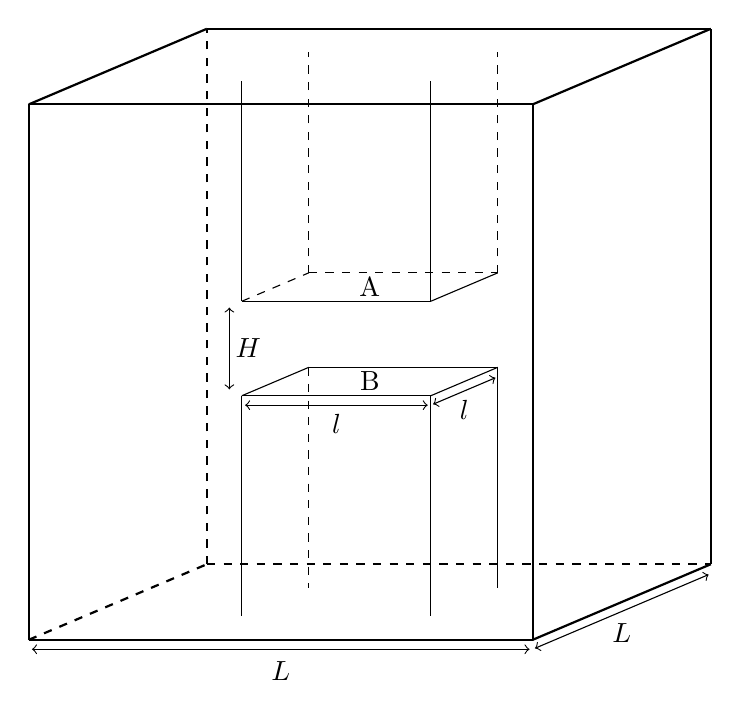
\begin{tikzpicture}[scale=.4, z={(-.707,-.3)}]
    \draw (6,0,0) -- (0,0,0);
    \draw (6,0,0) -- (6,0,-3);
    \draw (6,3,-3) -- (6,3,0);
    \draw (6,3,0) -- (0,3,0);
    \draw (0,0,-3) -- (6,0,-3);
    \draw (0,0,0) -- (0,0,-3); 
    \draw[dashed] (0,3,-3) -- (6,3,-3);
    \draw[dashed] (0,3,0) -- (0,3,-3);
    
    \draw (0,3,0) -- (0,10,0);
    \draw[dashed] (0,3,-3) -- (0,10,-3);
    \draw[dashed] (6,3,-3) -- (6,10,-3);
    \draw (6,3,0) -- (6,10,0);
    \draw (0,0,0) -- (0,-7,0);
    \draw[dashed] (0,0,-3) -- (0,-7,-3);
    \draw (6,0,-3) -- (6,-7,-3);
    \draw (6,0,0) -- (6,-7,0);
    
%    \draw (0,-7,0) -- (6,-7,0);
%    \draw (6,-7,0) -- (6,-7,-3);
    
    \draw[thick] (-5,10,2.5) -- (11,10,2.5);
    \draw[thick] (-5,10,-5.5) -- (11,10,-5.5);
    \draw[thick] (-5,10,2.5) -- (-5,10,-5.5);
    \draw[thick] (11,10,2.5) -- (11,10,-5.5);    
    \draw[thick] (-5,-7,2.5) -- (11,-7,2.5);
    \draw[thick,dashed] (-5,-7,-5.5) -- (11,-7,-5.5);
    \draw[thick,dashed] (-5,-7,2.5) -- (-5,-7,-5.5);
    \draw[thick] (11,-7,2.5) -- (11,-7,-5.5);
    \draw[thick] (-5,-7,2.5) -- (-5,10,2.5);    
    \draw[thick] (11,-7,2.5) -- (11,10,2.5);
    \draw[thick] (11,-7,-5.5) -- (11,10,-5.5);
    \draw[thick,dashed] (-5,-7,-5.5) -- (-5,10,-5.5);
    
    \draw[arrows=<->] (0.1,-0.3,0) -- (5.9,-0.3,0);
    \draw[] (3,-0.9,0) node{$l$};
    \draw[arrows=<->] (6,-0.3,-0.1) -- (6,-0.3,-2.9);
    \draw[] (6,-0.9,-1.5) node{$l$};
    \draw[arrows=<->] (-4.9,-7.3,2.5) -- (10.9,-7.3,2.5);
    \draw[] (3,-8.0,2.5) node{$L$};
    \draw[arrows=<->] (11,-7.3,2.4) -- (11,-7.3,-5.4);
    \draw[] (11,-8,-1.5) node{$L$};
    
    \draw (3,0,-1.5) node{B};
    \draw (3,3,-1.5) node{A};
    \draw[arrows=<->] (-0.4,0.2,0) -- (-0.4,2.8,0);
    \draw (0.2,1.5,0) node{$H$};
\end{tikzpicture}
\caption{Schematic structure of the finite plate system}
\end{figure}

\newpage
\section{Conclusion and Outlook}

\newpage
\section{Annex}
\myEqRef{diffusion_PDE}
\begin{align}
\rho(x,t) &= \frac{1}{\varepsilon\sqrt{2\pi\sfrac{t}{\delta t}}}\; e^{-\frac{x^2 \delta t}{2 \varepsilon^2 t}} \\
\frac{\partial}{\partial t} \rho(x,t) &= - \frac{1}{2t} \rho(x,t) + \frac{x^2 \delta t}{\varepsilon^2t^2} \rho(x,t) \\
&= \frac{1}{2} \left(\frac{x^2 \delta t}{\varepsilon^2t^2} - \frac{1}{t} \right)\rho(x,t) \\
\frac{\partial^2}{\partial x^2} \rho(x,t) &= \frac{\partial}{\partial x} \left(-\frac{x\delta t}{\varepsilon^2t} \right) \rho(x,t) \\
&= -\frac{\delta t}{\varepsilon^2t} \rho(x,t) + \frac{x^2\delta t^2}{\varepsilon^4 t^2} \rho(x,t) \\
&= \frac{\delta t}{\varepsilon^2}\left(\frac{x^2 \delta t}{\varepsilon^2 t^2} - \frac{1}{t}\right) \rho(x,t) \\
\frac{\partial}{\partial t} \rho(x,t) &= D \frac{\partial^2}{\partial x^2 } \rho(x,t)\\
\Rightarrow \frac{1}{2} &= D \cdot \frac{\delta t}{\varepsilon^2}\\
\Leftrightarrow D &= \frac{\varepsilon^2}{2\delta t}
\end{align}

\myEqRef{moivre_laplace_theorem}
\begin{align}
p(x,n) &= \binom{n}{k} \cdot 2^{-n}\;\;\;\; \mathrm{with}\;\;\; k = \frac{1}{2}\left(n+\frac{x}{\varepsilon}\right)\\
&= \frac{n!}{k!(n-k)!}\cdot 2^{-n}\\
\mathrm{with}\;\;\; n! &\cong \sqrt{2\pi n}\;n^ne^{-n}\tag{Stirling's\;formula}\\
\Rightarrow \;\;\; p(x,n) &\cong \frac{\sqrt{2\pi n}\;n^ne^{-n}}{\sqrt{2\pi k}\;k^ke^{-k} \sqrt{2\pi(n-k)}\;(n-k)^{n-k}e^{k-n}} \cdot 2^{-n}\\
&= \left(\frac{\sqrt{2\pi n}}{\sqrt{2\pi k}\;\sqrt{2\pi(n-k)}} \right) \underbrace{\left(\frac{e^{-n}}{e^{-k}\;e^{k-n}}\right)}_{=1} \left( \frac{n^n}{k^k(n-k)^{n-k}}\right)\cdot 2^{-n}\\
&= \sqrt{\frac{2n}{\pi(n+\sfrac{x}{\varepsilon})(n-\sfrac{x}{\varepsilon})}} \cdot \left(\frac{n}{2} \right)^k \cdot \left(\frac{n}{2} \right)^{n-k} \notag\\
&\;\;\;\;\cdot \left( \frac{1}{2}\left( n+\sfrac{x}{\varepsilon}\right) \right)^{-\frac{1}{2}(n+\sfrac{x}{\varepsilon})} \cdot \left( \frac{1}{2}\left( n-\sfrac{x}{\varepsilon}\right) \right)^{-\frac{1}{2}(n-\sfrac{x}{\varepsilon})} \\
&= \sqrt{\frac{2n}{\pi \left(n^2 - \left( \sfrac{x}{\varepsilon} \right)^2 \right)}} \cdot \left( \frac{n}{n+\sfrac{x}{\varepsilon}}\right)^{-\frac{1}{2}(n+\sfrac{x}{\varepsilon})} \cdot \left( \frac{n}{n-\sfrac{x}{\varepsilon}}\right)^{-\frac{1}{2}(n-\sfrac{x}{\varepsilon})} \\
&= \sqrt{\frac{2n}{\pi \left(n^2 - \left( \sfrac{x}{\varepsilon} \right)^2 \right)}} \cdot \left( 1 + \frac{x}{\varepsilon n}\right)^{-\frac{1}{2}(n+\sfrac{x}{\varepsilon})} \cdot \left( 1 - \frac{x}{\varepsilon n}\right)^{-\frac{1}{2}(n-\sfrac{x}{\varepsilon})} \\
\mathrm{use} \;\;\; x &= e^{\ln(x)}\\
\Rightarrow \;\;\; p(x,n) &\cong \sqrt{\frac{2}{\pi n\left(1 - \left( \frac{\sfrac{x}{\varepsilon}}{n} \right)^2 \right)}} \notag\\
&\;\;\;\;\cdot \exp\!\left\lbrace -\frac{n}{2}\left( 1+\frac{\sfrac{x}{\varepsilon}}{n} \right) \, \ln\!\left(1 + \frac{\sfrac{x}{\varepsilon}}{n} \right) -\frac{1}{2}(n-\sfrac{x}{\varepsilon})\, \ln\!\left(1 - \frac{\sfrac{x}{\varepsilon}}{n} \right) \right\rbrace \\
\mathrm{for}\;\;\; n &\rightarrow\infty \; \Rightarrow \; \alpha \rightarrow 0 \;\;\; \alpha := \frac{\sfrac{x}{\varepsilon}}{n}\; \\ 
&\Rightarrow\;\;  1-\alpha^2 \rightarrow 1 + ... \; \\
&\mathrm{and}\;\,\ln\!\left(1+\alpha\right) \rightarrow \alpha - \frac{1}{2}\alpha^2 + ... \\
\Rightarrow \;\;\; p(x,n) &\cong \sqrt{\frac{2}{n\pi}} \cdot \exp\!\left\lbrace-\frac{n}{2}\left[\left(1+\alpha\right)\left(\alpha - \frac{1}{2} \alpha^2 \right) +\left(1-\alpha\right)\left(-\alpha - \frac{1}{2} \alpha^2 \right)\right] \right\rbrace\\
&= \sqrt{\frac{2}{n\pi}} \cdot \exp\!\left\lbrace-\frac{n}{2}\left[\alpha -\frac{1}{2} \alpha^2 + \alpha^2 - \alpha - \frac{1}{2} \alpha^2 + \alpha^2 + \mathcal{O}(\alpha^3)\right] \right\rbrace \\
&\cong \sqrt{\frac{2}{n\pi}} \cdot \exp\!\left\lbrace-\frac{n}{2}\left[\alpha^2\right] \right\rbrace\\
&= \sqrt{\frac{2}{n\pi}} \cdot e^{-\sfrac{x^2}{2\varepsilon^2n}} 
\end{align}

\myEqRef{gauss_random_walk}
\begin{align}
p(x,n+1) &= \int_{-\infty}^\infty \frac{1}{\varepsilon\sqrt{2n\pi}}\, e^{-\sfrac{x'^2}{2n\varepsilon^2}} \cdot \frac{1}{\varepsilon\sqrt{2\pi}}\, e^{-\sfrac{(x - x')^2}{2\varepsilon^2}} \diff x'\\
&= \frac{1}{\varepsilon^2\sqrt{4\pi^2n}} \, \int_{-\infty}^\infty e^{-\frac{x'^2 + x^2n - 2xx'n +x'^2n}{2n\varepsilon^2}}\diff x' \\
&= \frac{1}{\varepsilon^2\sqrt{4\pi^2n}} \, \int_{-\infty}^\infty e^{-\frac{(n+1)x'^2 - 2xx'n + \sfrac{x^2n^2}{(n+1)} + x^2n - \sfrac{x^2n^2}{(n+1)}}{2n\varepsilon^2}}\diff x' \\
&= \frac{1}{\varepsilon^2\sqrt{4\pi^2n}} \, \int_{-\infty}^\infty e^{-\frac{(\sqrt{n+1}x - \sfrac{xn}{\sqrt{n+1}}')^2}{2n\varepsilon^2}} \cdot e^{- \frac{x^2 - \sfrac{x^2n}{(n+1)}}{2\varepsilon^2}}\diff x' \\
\mathrm{let}\;\;\; \alpha &= \frac{\sqrt{n+1}x' - \sfrac{xn}{\sqrt{n+1}}}{\sqrt{2n}\varepsilon}
\;\;\; \Rightarrow \;\;\diff\alpha = \sqrt{\frac{n+1}{2n\varepsilon^2}} \diff x' \notag\\
p(x,n+1) &= \frac{1}{\varepsilon^2\sqrt{4\pi^2n}} \sqrt{\frac{2n\varepsilon^2}{n+1}}\;\cdot\, e^{-\frac{(n+1)x^2 - x^2n}{2(n+1)\varepsilon^2}}\, \int_{-\infty}^\infty e^{-\alpha^2} \diff\alpha\notag\\
&= \frac{1}{\varepsilon\sqrt{2(n+1)\pi}}\;\cdot\, e^{-\frac{x^2}{2(n+1)\varepsilon^2}}\notag
\end{align}

\myEqRef{MSD}
\begin{align}
\langle x_n^2\rangle &= \int_{-\infty}^\infty x^2 \cdot \frac{1}{\varepsilon\sqrt{2\pi n}}\; e^{-\sfrac{x^2}{2\varepsilon^2 n}}\; \diff x\\
&= \frac{1}{\varepsilon\sqrt{2\pi n}} \; \int_{-\infty}^\infty x^2 \cdot e^{-\sfrac{x^2}{2\varepsilon^2 n}} \diff x \\
\mathrm{let}\;\;\; \alpha &= \frac{x}{\sqrt{2\varepsilon^2n}} \;\;\; \Rightarrow \;\;\; dx = \sqrt{2\varepsilon^2n}\diff\alpha\\
\langle x_n^2\rangle &= \frac{\sqrt{2\varepsilon^2n}}{\varepsilon\sqrt{2\pi n}} \; \int_{-\infty}^\infty 2 \varepsilon^2n\alpha^2\; e^{-\alpha^2} \diff\alpha\\
&= \frac{2\varepsilon^2n}{\sqrt{\pi}} \; \int_{-\infty}^\infty \alpha^2\; e^{-\alpha^2} \diff \alpha\\
&= \frac{\varepsilon^2n}{\sqrt{\pi}} \; \int_{-\infty}^\infty \alpha \cdot 2\alpha\; e^{-\alpha^2}\; \diff\alpha\\
&= \frac{\varepsilon^2n}{\sqrt{\pi}} \; \left(\left.-\alpha e^{-\alpha^2}\;\; \right|_{-\infty}^\infty \;\;\; - \int_{-\infty}^\infty 1 \cdot \left(-e^{-\alpha^2} \right) \diff\alpha\right) \\
&= \frac{\varepsilon^2n}{\sqrt{\pi}} \; \left(0 + \sqrt{\pi} \right)\\
&= \varepsilon^2 n \\
&= 2 D \delta t n \\
&= 2 D t
\end{align}

\newpage
\printbibliography 
\end{document}